\documentclass[letterpaper]{article}
\usepackage[cmyk]{xcolor}
\usepackage{amssymb}
\usepackage{tikz}

\begin{document}

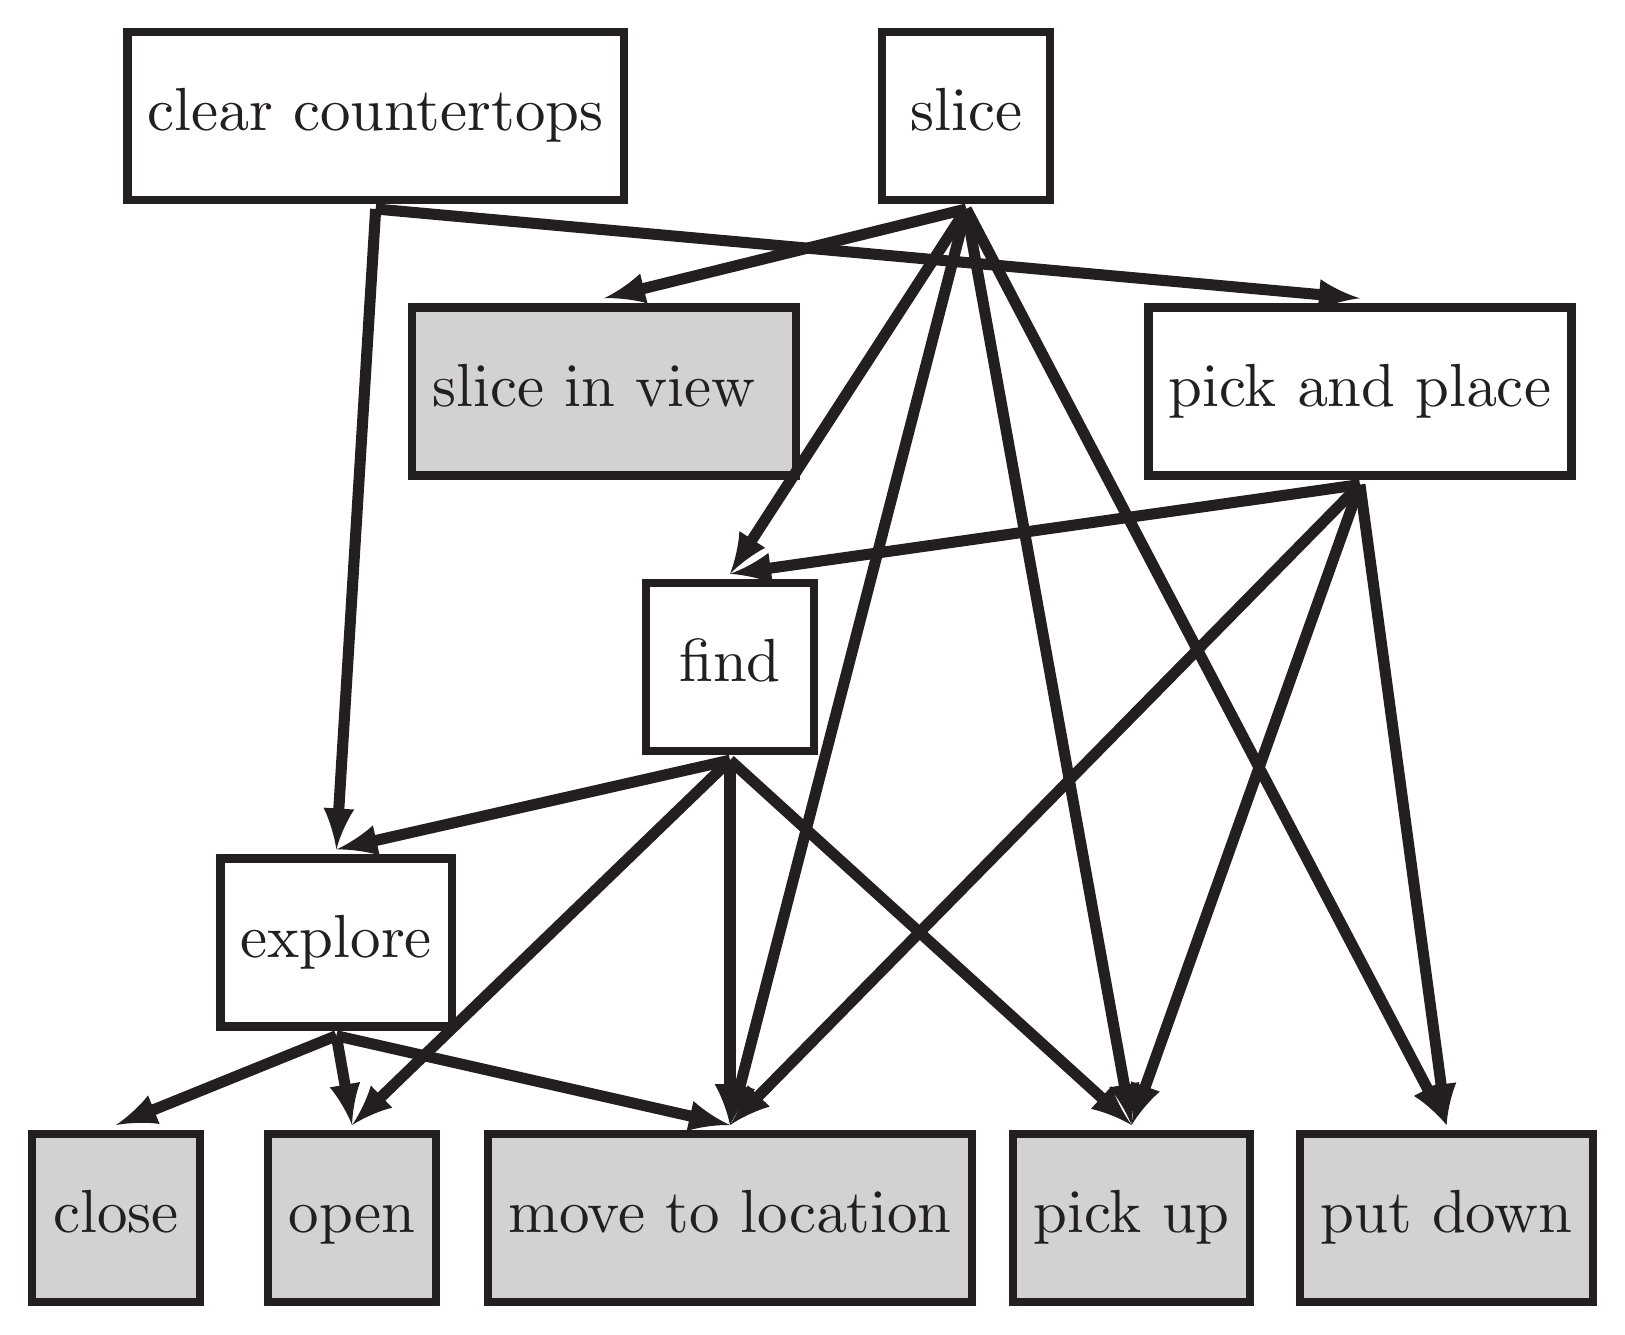
\begin{tikzpicture}[
    graynode/.style={rectangle, draw=black, fill=gray!40!white, very thick, minimum size=0.08\columnwidth, scale=2.2, line width=3pt, },
    whitenode/.style={rectangle, draw=black, fill=white, very thick, minimum size=0.08\columnwidth, scale=2.2, line width=3pt, },
]

    \node[graynode] (close) at (1.2, 1) { close\strut };
    \node[graynode] (open) at (4.2, 1) { open\strut };
    \node[graynode] (move) at (9, 1) { move to location\strut };
    \node[graynode] (pick) at (14.1, 1) { pick up\strut };
    \node[graynode] (put) at (18.1, 1) { put down\strut };

    \node[whitenode] (explore) at (4, 4.5) { explore\strut };
    \node[whitenode] (find) at (9, 8) { find\strut };
    \node[graynode] (sliceb) at (7.4, 11.5) { slice in view \strut };
    \node[whitenode] (pandp) at (17, 11.5) { pick and place\strut };
    \node[whitenode] (clear) at (4.5, 15) { clear countertops\strut };
    \node[whitenode] (slice) at (12, 15) { slice\strut };

    \draw[-latex, line width=4pt] (explore.south) -- (close.north);
    \draw[-latex, line width=4pt] (explore.south) -- (open.north);
    \draw[-latex, line width=4pt] (explore.south) -- (move.north);
    \draw[-latex, line width=4pt] (find.south) -- (explore.north);
    \draw[-latex, line width=4pt] (find.south) -- (move.north);
    \draw[-latex, line width=4pt] (find.south) -- (pick.north);
    \draw[-latex, line width=4pt] (find.south) -- (open.north);
    \draw[-latex, line width=4pt] (pandp.south) -- (find.north);
    \draw[-latex, line width=4pt] (pandp.south) -- (pick.north);
    \draw[-latex, line width=4pt] (pandp.south) -- (put.north);
    \draw[-latex, line width=4pt] (pandp.south) -- (move.north);
    \draw[-latex, line width=4pt] (slice.south) -- (pick.north);
    \draw[-latex, line width=4pt] (slice.south) -- (find.north);
    \draw[-latex, line width=4pt] (slice.south) -- (move.north);
    \draw[-latex, line width=4pt] (slice.south) -- (sliceb.north);
    \draw[-latex, line width=4pt] (slice.south) -- (put.north);
    \draw[-latex, line width=4pt] (clear.south) -- (pandp.north);
    \draw[-latex, line width=4pt] (clear.south) -- (explore.north);
\end{tikzpicture}

\end{document}